% IEEE conference paper: QAOA-Based Economic Load Dispatch Using QUBO Formulation
% Compile on Overleaf with pdfLaTeX (upload the whole paper/ folder).
\documentclass[conference]{IEEEtran}

\usepackage{amsmath,amssymb}
\usepackage{graphicx}
\usepackage{booktabs}
\usepackage{cite}
\usepackage[hidelinks]{hyperref}

\graphicspath{{figures/}}
\newcommand{\PD}{P_{\mathrm{D}}}
\newcommand{\PL}{P_{\mathrm{L}}}

\begin{document}

\title{QAOA-Based Economic Load Dispatch Using QUBO Formulation on a 6-Bus System}

\author{\IEEEauthorblockN{J. Karthikeya, A. Krishna Chaitanya, N. Ramesh, M. Harika, and B. Madhusudhan Rao}
\IEEEauthorblockA{Department of Electrical and Electronics Engineering\\
Rajiv Gandhi University of Knowledge Technologies (RGUKT), Nuzvid, Andhra Pradesh, India}}

\maketitle

\begin{abstract}
Economic load dispatch (ELD) of the 6-bus, 3-generator Wood--Wollenberg system is formulated as a 12-variable quadratic unconstrained binary optimization (QUBO) problem and solved with the quantum approximate optimization algorithm (QAOA) for all 12 periods of a daily load profile (180--330~MW). Generator outputs are encoded with four bits per unit, so the limits hold by construction; the power balance is a quadratic penalty whose weight is chosen by a sweep. A conditional value-at-risk (CVaR) objective with layer-wise interpolated initialization trains the circuit, and the five best sampled dispatches are refined with SLSQP inside a one-step box. The hybrid dispatch is within 0.041\,\% of the SLSQP optimum in every period, and the trained circuit at depth $p = 4$ samples the optimal bitstring 10.2 times more often than uniform sampling (up to 31 times). On the same QUBO with the same budget, QAOA succeeded in 100\,\% of 240 runs against 92.5\,\% for simulated annealing. On the IBM \texttt{ibm\_marrakesh} processor a 6-qubit instance retained about 90\,\% of the ideal gain. With network-derived loss coefficients the method stays within 0.08\,\% of the loss-inclusive optimum, and a Newton--Raphson load flow confirms voltages and reactive power but reveals a line overload of up to 145\,\% that the classical optimum shares. No computational speed-up is claimed.
\end{abstract}

\begin{IEEEkeywords}
Economic load dispatch, QAOA, QUBO, Ising model, quantum computing, CVaR, simulated annealing, particle swarm optimization.
\end{IEEEkeywords}

\section{Introduction}
Economic load dispatch allocates the demand among committed generators at minimum fuel cost subject to power balance and unit limits \cite{wood2014}. For quadratic costs the problem is convex and is solved exactly by $\lambda$-iteration or nonlinear programming; heuristics such as particle swarm optimization (PSO) \cite{gaing2003} are used when costs are non-convex.

Quantum optimization offers a different route: an optimization problem written as a QUBO maps to an Ising Hamiltonian \cite{lucas2014}, whose low-energy states QAOA \cite{farhi2014} tries to prepare. Quantum and quantum-inspired methods have been proposed for dispatch \cite{han2024,jing2023,wang2024}, but results are seldom compared with exact and heuristic baselines on a common criterion or checked with an AC load flow.

This paper contributes: (i) a transparent ELD-to-QUBO formulation with a justified penalty weight; (ii) a measurement of QAOA accuracy and probability amplification against the exact optimum over a full 12-period profile; (iii) a fair comparison with simulated annealing (SA), PSO and genetic algorithms (GA) under one success criterion; (iv) a real-hardware run on an IBM Heron processor; and (v) an extension to transmission losses validated by a Newton--Raphson (NR) load flow. Code and data are public.\footnote{\url{https://github.com/Karthik73965/eld-qaoa}}

\section{Problem Formulation}
\subsection{Economic load dispatch}
For $N$ units with cost $C_i(P_i) = a_iP_i^2 + b_iP_i + c_i$,
\begin{equation}
\min_{P} \sum_{i=1}^{N} C_i(P_i) \ \ \text{s.t.}\ \ \sum_{i=1}^{N} P_i = \PD,\ \ P_i^{\min} \le P_i \le P_i^{\max}.
\label{eq:eld}
\end{equation}
The test system is the 6-bus, 3-generator system of \cite{wood2014} with the generator, load and line data of Prada \cite[App.~D]{prada2017}; the 100~MVA base and voltage set-points are from MATPOWER \texttt{case6ww} \cite{matpower2011}. Table~\ref{tab:gen} lists the units. The 12 period demands are 250, 210, 190, 180, 200, 230, 270, 310, 330, 320, 300 and 270~MW. SLSQP \cite{kraft1988} gives the reference optimum, confirmed by $\lambda$-iteration to $10^{-6}$~\$/h; the daily optimal cost is \$43{,}171.05.

\begin{table}[t]
\centering
\caption{Generator Data \cite{prada2017}}
\label{tab:gen}
\setlength{\tabcolsep}{3.5pt}
\begin{tabular}{lcccccc}
\toprule
Unit & Bus & $P^{\min}$ & $P^{\max}$ & $a$ & $b$ & $c$\\
 & & (MW) & (MW) & (\$/MW$^2$h) & (\$/MWh) & (\$/h)\\
\midrule
G1 & 1 & 50.0 & 200 & 0.00533 & 11.669 & 213.1\\
G2 & 2 & 37.5 & 150 & 0.00889 & 10.333 & 200.0\\
G3 & 3 & 45.0 & 180 & 0.00741 & 10.833 & 240.0\\
\bottomrule
\end{tabular}
\end{table}

\subsection{Binary encoding and QUBO}
Each output uses $n = 4$ bits,
\begin{equation}
P_i(x) = P_i^{\min} + \Delta P_i \sum_{k=0}^{n-1} 2^k x_{ik},\quad \Delta P_i = \frac{P_i^{\max} - P_i^{\min}}{2^n - 1},
\label{eq:enc}
\end{equation}
giving steps of 10, 7.5 and 9~MW, 12 binary variables and 4096 candidate dispatches. Every bitstring respects the limits, so only the balance needs a penalty:
\begin{equation}
E(x) = \sum_{i} C_i\big(P_i(x)\big) + A\Big(\sum_i P_i(x) - \PD\Big)^2.
\label{eq:qubo}
\end{equation}
Since $P_i(x)$ is linear in $x$, $E$ is quadratic in the bits. An exhaustive sweep over $A \in \{1, 5, 20, 100\}$ in all periods gave maximum QUBO-optimum mismatches of 7.0, 2.0, 0.5 and 0~MW, with mean cost differences of $-2.00$, $-0.39$, $+0.011$ and $+0.176$\,\%; negative values come from under-supply. $A = 20$ is the smallest weight that keeps the mismatch within 0.5~MW and is used throughout.

\subsection{Ising Hamiltonian}
With $x_j = (1 - Z_j)/2$, \eqref{eq:qubo} becomes $H_C = \sum_j h_j Z_j + \sum_{j<l} J_{jl} Z_jZ_l$ plus a constant, with 12 linear and 66 coupling terms (the penalty couples every pair of bits). The identity $E(x) = \langle x|H_C|x\rangle + \text{const}$ was verified for all 4096 states.

\section{Hybrid QAOA Method}
\subsection{Circuit}
Depth-$p$ QAOA prepares $\prod_{\ell=1}^{p} e^{-i\beta_\ell H_M} e^{-i\gamma_\ell H_C}|+\rangle^{\otimes 12}$ with $H_M = \sum_j X_j$, implemented with $R_Z$ and $R_{ZZ}$ gates for the cost layer and $R_X$ gates for the mixer. $H_C$ is scaled by its largest coefficient.

\subsection{Training}
The parameters minimize the CVaR of the energy distribution with $\alpha = 0.05$ \cite{barkoutsos2020}, which rewards probability on the best states rather than a good mean. COBYLA (400 iterations) is used, with 8 random starts at $p = 1$ and INTERP initialization \cite{zhou2020} for $p = 2$--4. Training uses the exact statevector in Qiskit \cite{qiskit}.

\subsection{Sampling and refinement}
The trained circuit is sampled with 4096 shots. The five lowest-energy distinct bitstrings are decoded and each is refined by SLSQP with every unit allowed to move at most $\pm\Delta P_i$, enforcing exact balance. The cheapest refined dispatch is the result. The refinement searches only the cell chosen by QAOA, so its quality depends on QAOA finding the right cell.

\subsection{Measures}
The cost gap is relative to SLSQP. Amplification is the probability of the QUBO-optimal bitstring divided by $1/4096$. A shot is near-optimal if its dispatch is within one grid step of $\PD$ and its cost within 1\,\% of SLSQP. A run succeeds if its final cost is within 0.1\,\% of SLSQP with $|\text{mismatch}| \le 0.01$~MW.

\section{Results}
\subsection{Hybrid dispatch}
Fig.~\ref{fig:dispatch} shows the 12-period dispatch at $p = 4$. QAOA sampled the exact QUBO optimum in all 12 periods. After refinement every dispatch meets demand exactly; the worst gap is 0.040\,\% (period 5) and the daily cost is \$43{,}173.88, \$2.83 above the optimum. Exhaustive search with the same refinement gives identical costs, so the residual gap is set by the 4-bit grid and the refinement box, not by QAOA: in period 5 the QUBO optimum (60, 67.5, 72)~MW is more than one step from the SLSQP optimum (50, 83.5, 66.5)~MW.

\begin{figure}[t]
\centering
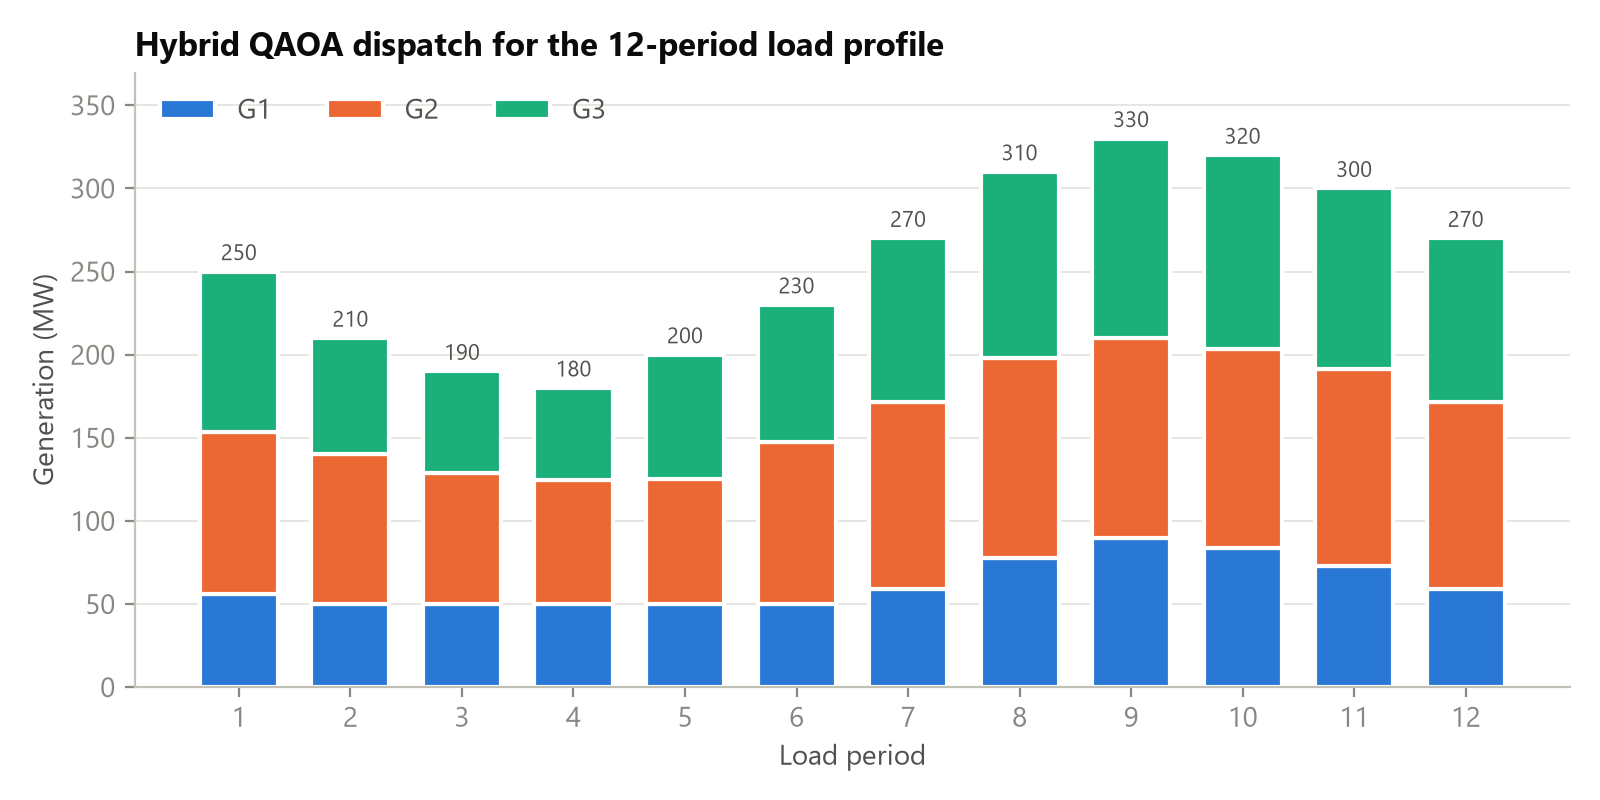
\includegraphics[width=\columnwidth]{dispatch_by_period}
\caption{Hybrid QAOA dispatch for 12 periods ($p = 4$, 4096 shots).}
\label{fig:dispatch}
\end{figure}

\subsection{Effect of depth}
Table~\ref{tab:depth} and Fig.~\ref{fig:amp} show that amplification grows steadily with depth, from 4.6 at $p = 1$ to 10.2 at $p = 4$. At $p = 4$, 20.4\,\% of shots are near-optimal against 3.1\,\% for uniform sampling. Amplification varies by period, from 2.4 (period 6) to 31.0 (period 4).

\begin{table}[t]
\centering
\caption{QAOA Performance Versus Depth (Mean of 12 Periods)}
\label{tab:depth}
\setlength{\tabcolsep}{4pt}
\begin{tabular}{ccccc}
\toprule
$p$ & Ampl.\ mean & Ampl.\ max & P(near-opt.) & Train (s)\\
\midrule
1 & 4.58 & 15.1 & 10.4\,\% & 3.5\\
2 & 6.76 & 21.3 & 13.9\,\% & 4.0\\
3 & 8.33 & 25.5 & 16.8\,\% & 6.3\\
4 & 10.18 & 31.0 & 20.4\,\% & 8.2\\
Random & 1 & 1 & 3.1\,\% & --\\
\bottomrule
\end{tabular}
\end{table}

\begin{figure}[t]
\centering
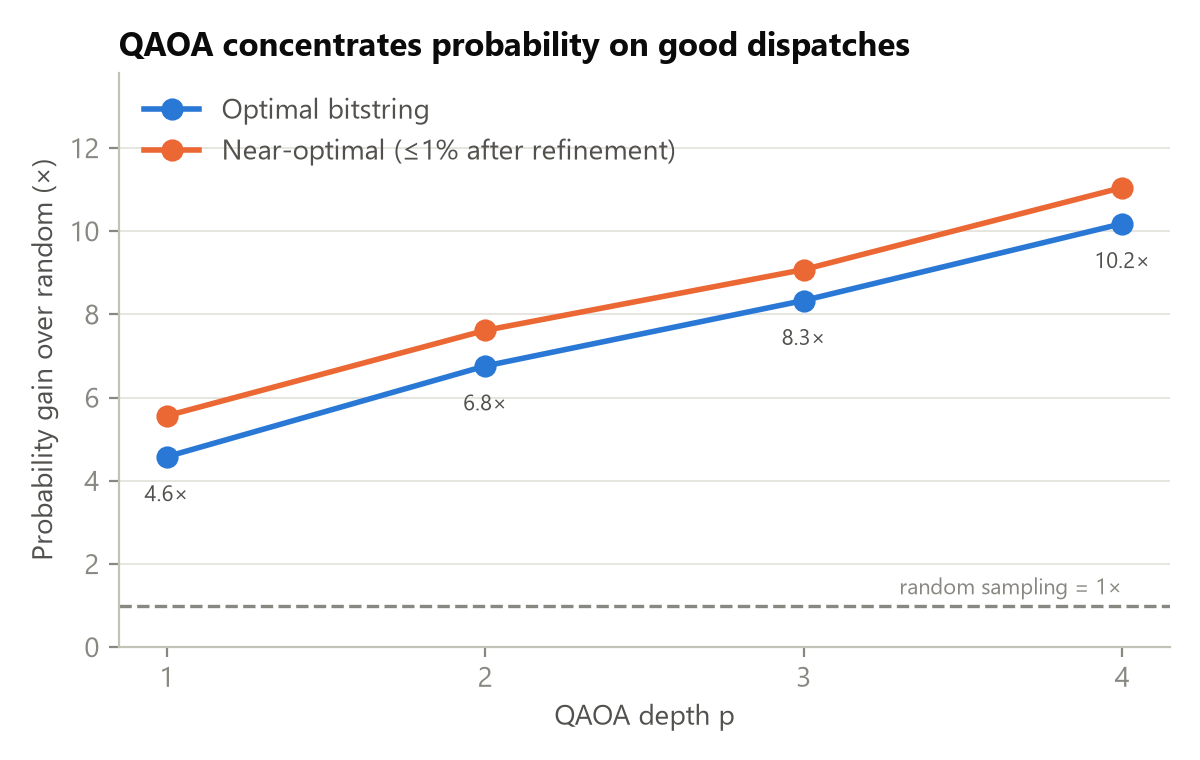
\includegraphics[width=0.85\columnwidth]{amplification_vs_depth}
\caption{Gain in probability of the optimal bitstring over uniform sampling.}
\label{fig:amp}
\end{figure}

\subsection{Comparison with standard algorithms}
Each stochastic method was run with 20 seeds per period (240 runs). Exhaustive search, SA \cite{kirkpatrick1983} and QAOA all evaluate 4096 bitstrings of the same QUBO and refine their five best in the same way. PSO \cite{shi1998} and real-coded GA with SBX \cite{deb1995} work on the continuous outputs (3030 evaluations) with either a penalty ($10^4\cdot$mismatch$^2$) or the dependent-unit method of Gaing \cite{gaing2003}. Table~\ref{tab:compare} and Fig.~\ref{fig:base} give the results.

\begin{table}[t]
\centering
\caption{Comparison Over 240 Runs (Success: Within 0.1\,\% of SLSQP and Balanced)}
\label{tab:compare}
\setlength{\tabcolsep}{4pt}
\begin{tabular}{lrrrr}
\toprule
Method & Mean gap & Worst gap & Success & Time\\
\midrule
PSO, dependent unit & 0.000\,\% & 0.000\,\% & 100\,\% & 13 ms\\
GA, dependent unit & 0.000\,\% & 0.000\,\% & 100\,\% & 80 ms\\
PSO, penalty & 0.645\,\% & 2.190\,\% & 13.8\,\% & 10 ms\\
GA, penalty & 0.763\,\% & 3.011\,\% & 7.5\,\% & 81 ms\\
Exhaustive + refine & 0.007\,\% & 0.040\,\% & 100\,\% & 10 ms\\
SA + refine & 0.029\,\% & 0.437\,\% & 92.5\,\% & 71 ms\\
\textbf{QAOA + refine} & \textbf{0.007\,\%} & \textbf{0.040\,\%} & \textbf{100\,\%} & 0.28 s$^{*}$\\
\bottomrule
\multicolumn{5}{l}{\footnotesize $^{*}$Simulated sampling, after about 22~s of training per period.}
\end{tabular}
\end{table}

\begin{figure}[t]
\centering
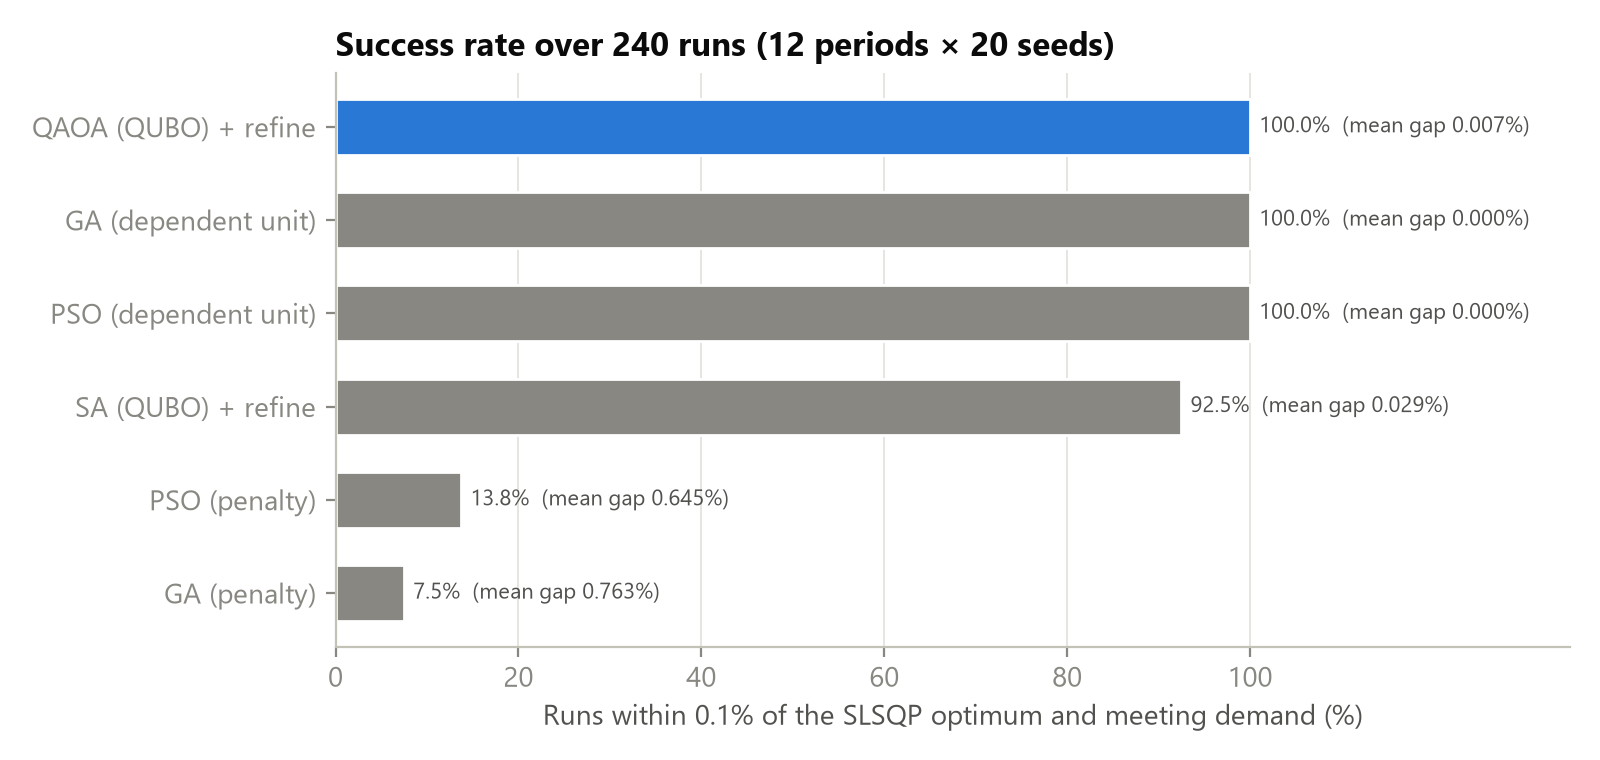
\includegraphics[width=\columnwidth]{baselines_success}
\caption{Success rate of the stochastic methods over 240 runs.}
\label{fig:base}
\end{figure}

On the same binary problem, QAOA matched exhaustive search in every run, while SA with the same budget and refinement failed in 7.5\,\% of runs (worst gap 0.44\,\%). Continuous heuristics reach the exact optimum when balance is handled by the dependent-unit method but often stall with a penalty, which shows that constraint handling matters as much as the algorithm. Every classical method is faster than simulated QAOA; SLSQP takes about 1~ms.

\subsection{IBM quantum hardware}
Period 1 was run at $p = 1$ with 4096 shots on \texttt{ibm\_marrakesh}, a 156-qubit IBM Heron processor (Table~\ref{tab:hw}, Fig.~\ref{fig:hw}). With 2 bits per unit (6 qubits, 46 two-qubit gates after transpilation) the hardware found the optimal bitstring 2.4 times more often than random, retaining about 90\,\% of the simulator's probability, and the refined dispatch equals the SLSQP optimum. With 3 bits per unit (9 qubits, 144 two-qubit gates) noise reduced the gain to 1.2, although the near-optimal probability (15.5\,\% against 6.1\,\%) still shows a clear signal.

\begin{table}[t]
\centering
\caption{IBM Hardware Results, Period 1 (250 MW), $p = 1$}
\label{tab:hw}
\setlength{\tabcolsep}{3pt}
\small
\begin{tabular}{lcc}
\toprule
 & 6 qubits & 9 qubits\\
\midrule
Depth / two-qubit gates & 124 / 46 & 271 / 144\\
P(opt.): rand./HW/sim. & 1.56/3.69/4.11\,\% & 0.20/0.24/0.53\,\%\\
P(near): rand./HW/sim. & 12.5/18.9/24.2\,\% & 6.1/15.5/18.0\,\%\\
Hybrid cost gap & 0.000\,\% & 0.254\,\%\\
\bottomrule
\end{tabular}
\end{table}

\begin{figure}[t]
\centering
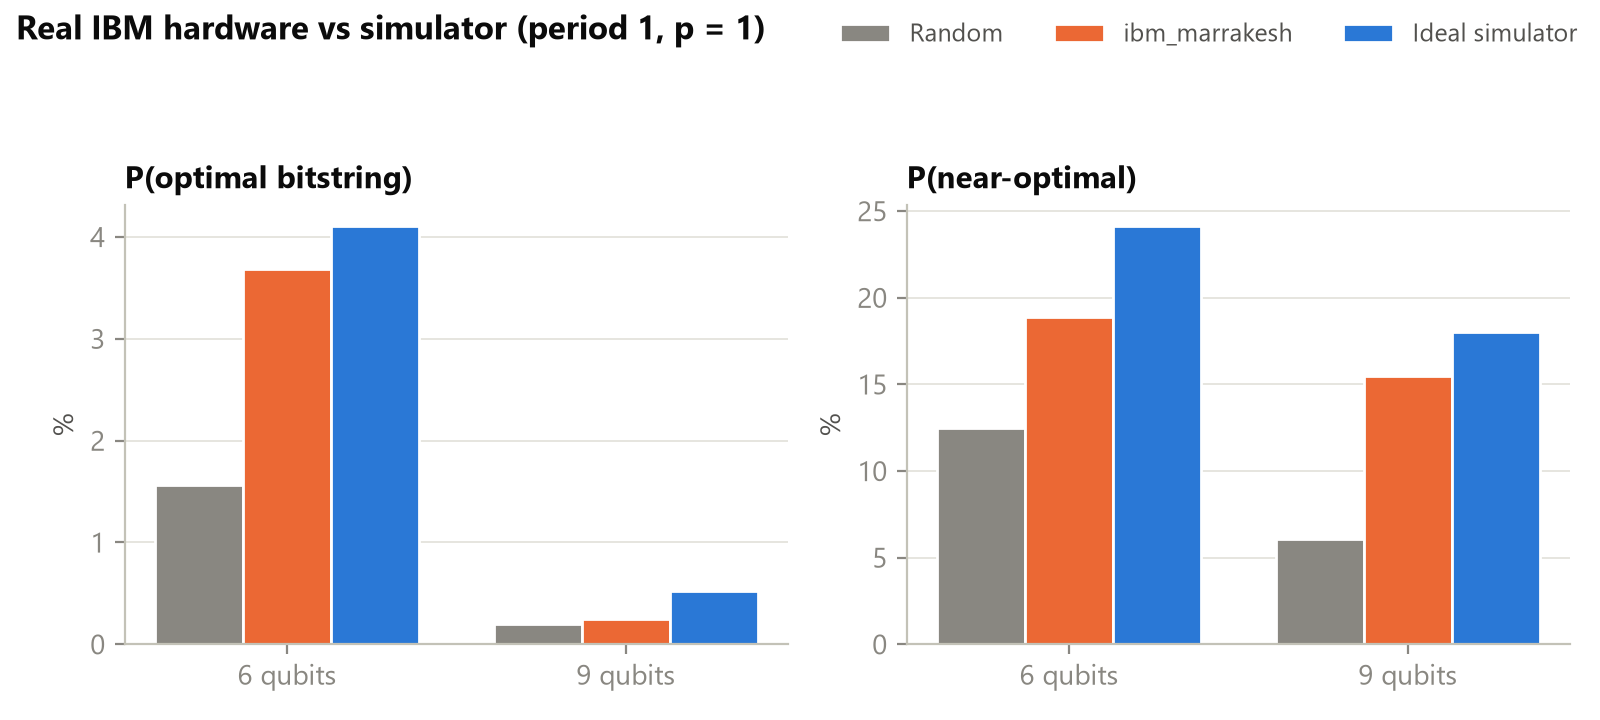
\includegraphics[width=\columnwidth]{ibm_hardware}
\caption{Real hardware against the ideal simulator and uniform sampling.}
\label{fig:hw}
\end{figure}

\section{Losses and AC Validation}
\subsection{Loss model and method}
B-coefficients are derived from the line data: with bus 1 as slack, DC power-transfer distribution factors give the line flows, and $\sum_\ell r_\ell f_\ell^2$ expands into Kron's formula $\PL = P^\top BP + B_0^\top P + B_{00}$ \cite{wood2014}. Because the QUBO must remain quadratic, an outer loop solves the QUBO for $\PD + \PL^{(k)}$ with QAOA ($p = 3$), refines with the loss-inclusive balance, and updates $\PL$; it converged in 2--3 rounds. Every dispatch is checked with a polar NR load flow, validated against PYPOWER on \texttt{case6ww} (identical slack output, losses, reactive powers, voltages and angles); NR converged in 4 iterations in every case.

\subsection{Results}
Losses of 2.7--9.2~MW raise the optimal cost by 1.2--2.6\,\% per period and 2.0\,\% over the day. The hybrid dispatch stays within 0.08\,\% of the loss-inclusive SLSQP optimum. The formula overestimates the AC losses by 1.5--4.3\,\% (Fig.~\ref{fig:loss}), so the AC slack produces 0.07--0.22~MW less than scheduled. Bus voltages remain within 1.009--1.070~pu and reactive outputs within limits.

Line T09 (bus 3--6), however, exceeds its 60~MVA rating in periods 1 and 7--12 and its 75~MVA short-term rating in periods 8--11, reaching 145\,\% at the 330~MW peak (Fig.~\ref{fig:line}). The SLSQP optimum gives the same overloads (142.7\,\% at the peak), so the cause is that ELD ignores line limits, not the quantum method.

\begin{figure}[t]
\centering
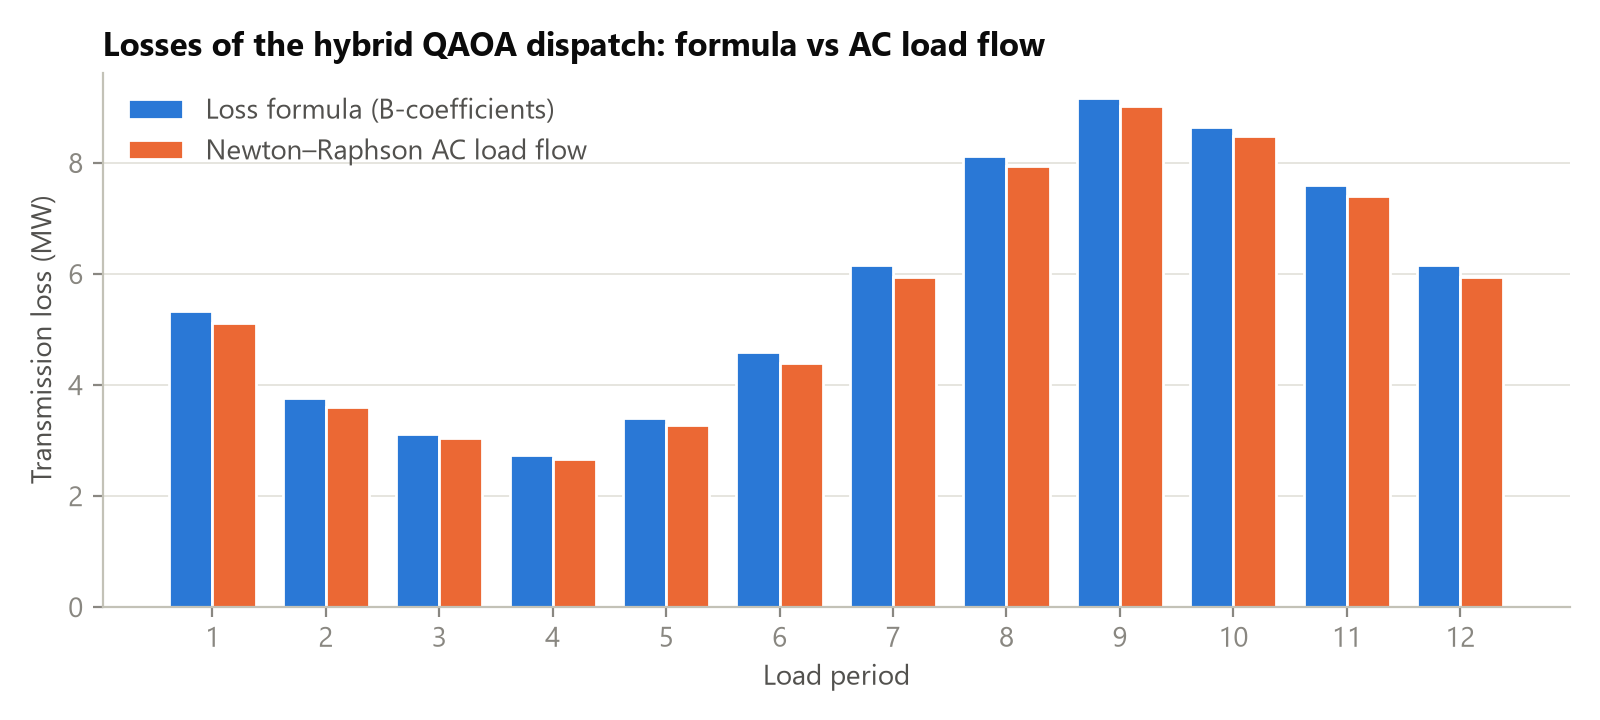
\includegraphics[width=\columnwidth]{losses}
\caption{Losses of the hybrid dispatch: B-coefficient formula against NR load flow.}
\label{fig:loss}
\end{figure}

\begin{figure}[t]
\centering
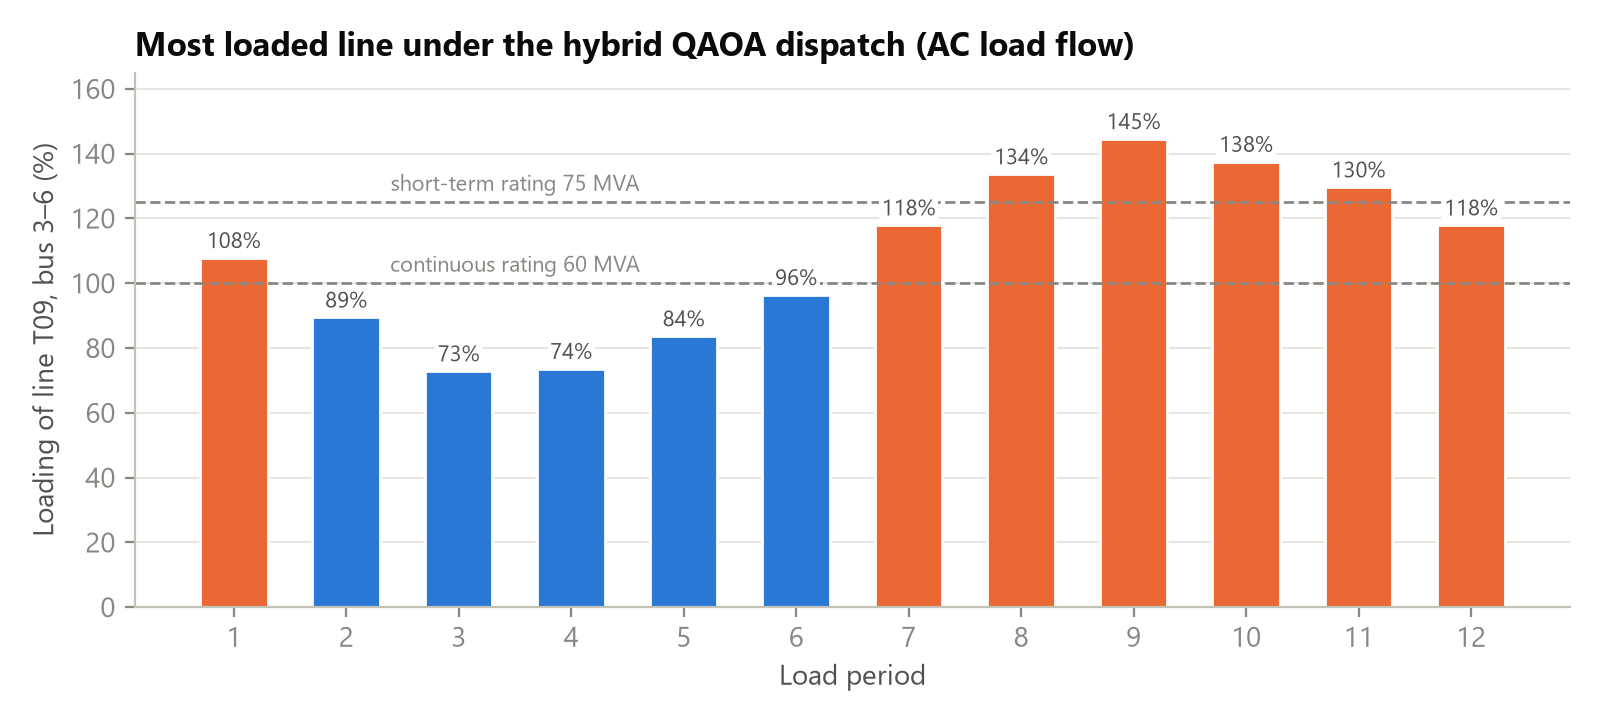
\includegraphics[width=\columnwidth]{line_loading}
\caption{Loading of line T09 under the hybrid dispatch (AC load flow).}
\label{fig:line}
\end{figure}

\section{Discussion}
The hybrid method is accurate, and the circuit concentrates probability on good dispatches in a way that grows with depth and partly survives on present hardware. It is not fast: for a convex three-unit problem, classical solvers need milliseconds, while simulating QAOA costs time that grows exponentially with qubits. The 4-bit grid also requires classical refinement. The value of the QUBO route lies in problems that are binary by nature, such as unit commitment, where classical methods face combinatorial growth.

\section{Conclusion}
ELD of the 6-bus system was solved as a 12-qubit QUBO with CVaR-trained QAOA and a bounded classical refinement. The hybrid dispatch was within 0.041\,\% of the optimum in all 12 periods, the optimal bitstring was amplified 10.2 times on average at $p = 4$, and QAOA outperformed SA on the same QUBO (100\,\% against 92.5\,\% success). A 6-qubit instance ran successfully on IBM hardware. With losses the method stayed within 0.08\,\% of the optimum, and AC validation exposed a line overload shared by the classical optimum. Future work includes security-constrained dispatch with line-flow penalties, unit commitment, larger IEEE test systems and error mitigation for larger hardware runs.

\begin{thebibliography}{99}
\bibitem{wood2014} A.~J. Wood, B.~F. Wollenberg, and G.~B. Sheblé, \emph{Power Generation, Operation, and Control}, 3rd~ed. Hoboken, NJ, USA: Wiley, 2014.
\bibitem{gaing2003} Z.-L. Gaing, ``Particle swarm optimization to solving the economic dispatch considering the generator constraints,'' \emph{IEEE Trans. Power Syst.}, vol.~18, no.~3, pp.~1187--1195, Aug. 2003.
\bibitem{lucas2014} A.~Lucas, ``Ising formulations of many NP problems,'' \emph{Front. Phys.}, vol.~2, art.~5, 2014.
\bibitem{farhi2014} E.~Farhi, J.~Goldstone, and S.~Gutmann, ``A quantum approximate optimization algorithm,'' arXiv:1411.4028, 2014.
\bibitem{han2024} X.~Han, Z.~Li, and Y.~Xu, ``Quantum assisted stochastic economic dispatch for renewables rich power systems,'' arXiv:2404.13073, 2024.
\bibitem{jing2023} H.~Jing, Y.~Wang, and Y.~Li, ``Data-driven quantum approximate optimization algorithm for power systems,'' \emph{Commun. Eng.}, vol.~2, art.~12, 2023.
\bibitem{wang2024} M.~Wang, Z.~Cao, and Y.~Li, ``Quantum-behaved particle swarm optimization based on concentration selection probability assignment weights for power system economic dispatch,'' \emph{IEEJ Trans. Electr. Electron. Eng.}, vol.~19, no.~5, pp.~640--652, 2024.
\bibitem{prada2017} J.~F. Prada, ``Ensuring the reliable operation of the power grid: State-based and distributed approaches to scheduling energy and contingency reserves,'' Ph.D. dissertation, Carnegie Mellon Univ., Pittsburgh, PA, USA, 2017.
\bibitem{matpower2011} R.~D. Zimmerman, C.~E. Murillo-Sánchez, and R.~J. Thomas, ``MATPOWER: Steady-state operations, planning, and analysis tools for power systems research and education,'' \emph{IEEE Trans. Power Syst.}, vol.~26, no.~1, pp.~12--19, Feb. 2011.
\bibitem{kraft1988} D.~Kraft, ``A software package for sequential quadratic programming,'' DFVLR, Tech. Rep. DFVLR-FB 88-28, 1988.
\bibitem{barkoutsos2020} P.~Kl. Barkoutsos, G.~Nannicini, A.~Robert, I.~Tavernelli, and S.~Woerner, ``Improving variational quantum optimization using CVaR,'' \emph{Quantum}, vol.~4, p.~256, 2020.
\bibitem{zhou2020} L.~Zhou, S.-T. Wang, S.~Choi, H.~Pichler, and M.~D. Lukin, ``Quantum approximate optimization algorithm: Performance, mechanism, and implementation on near-term devices,'' \emph{Phys. Rev. X}, vol.~10, 021067, 2020.
\bibitem{qiskit} Qiskit contributors, ``Qiskit: An open-source framework for quantum computing,'' 2026. [Online]. Available: \url{https://github.com/Qiskit/qiskit}
\bibitem{kirkpatrick1983} S.~Kirkpatrick, C.~D. Gelatt~Jr., and M.~P. Vecchi, ``Optimization by simulated annealing,'' \emph{Science}, vol.~220, no.~4598, pp.~671--680, 1983.
\bibitem{shi1998} Y.~Shi and R.~Eberhart, ``A modified particle swarm optimizer,'' in \emph{Proc. IEEE Int. Conf. Evol. Comput.}, 1998, pp.~69--73.
\bibitem{deb1995} K.~Deb and R.~B. Agrawal, ``Simulated binary crossover for continuous search space,'' \emph{Complex Syst.}, vol.~9, pp.~115--148, 1995.
\end{thebibliography}

\end{document}
